\chapter{Working environment}

\section{COOLFluiD}

\subsection{What is \cf ?}

\cf is a CSE (\textit{\textbf{C}ollaborative \textbf{S}imulation
\textbf{E}nvironment}) for complex multiphysics simulations. A CSE is a set of
independant components that can collaborate to form a simulation.\\

\cf is composed of a kernel and around a hundred of plug-ins that can
collaborate to form a simulation. Each plug-in is a physical model or a
numerical method such as solvers, equations, mesh formats,... . A physical
model is a mathematical model programmed to simulate a given physics problem.
The kernel combines these plug-ins together at runtime to solve a specific
problem. This makes \cf extremely flexible.\\

The project, began in 2002, is led by Doctor Tiago Quintino. It has 12
permanent European developers (all of them are scientists) and the Institute
hosts many European stagiaires that collaborate to the project. Many other
European partners, such as university research groups, specialized in certain
fields, contribute to the project by giving their knowledge.\\

\subsection{Application examples}

Below, a figure presenting the deformation of an aiplane wing under the
effects of the air flow around it. Both solutions of flow and wing structure
are managed by independant components that collaborate with each other to form
the overall simulation.

\begin{figure}[H]
 \begin{center}
  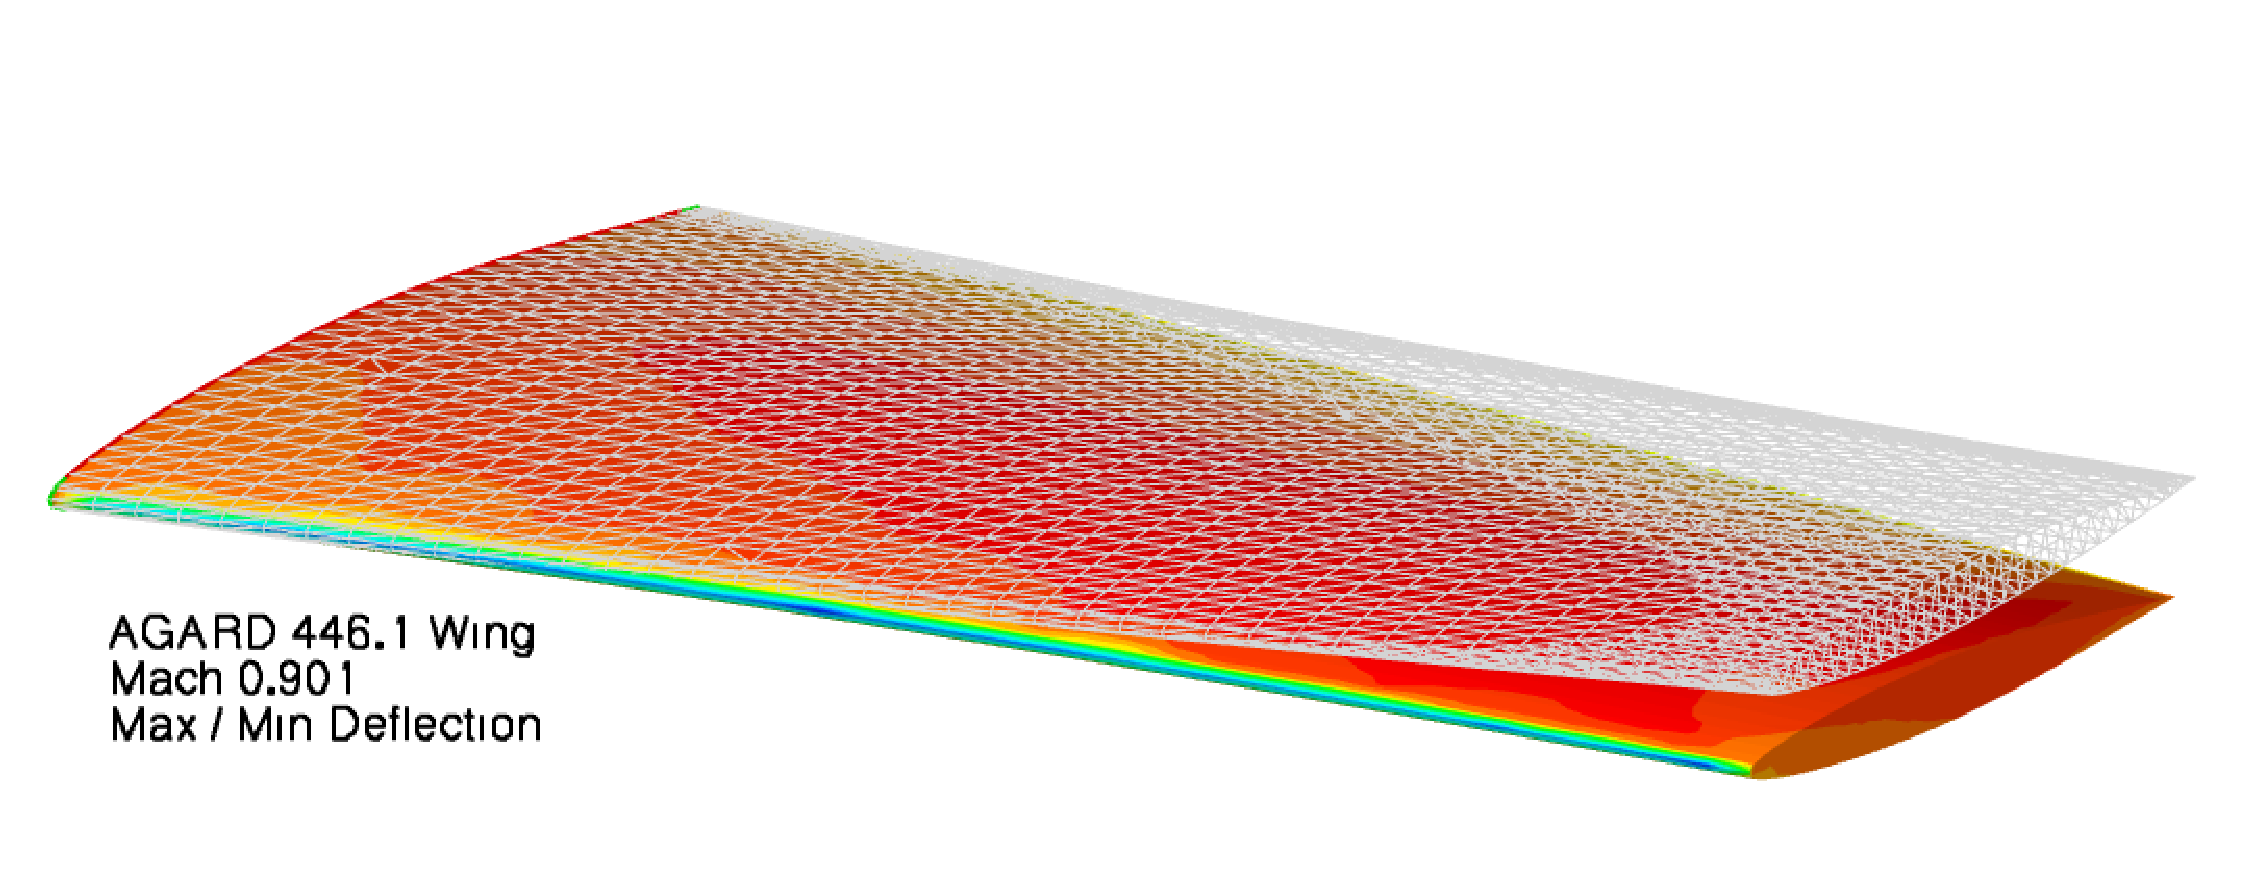
\includegraphics[width=0.95\textwidth]{images/agard_wing}
 \end{center}
\caption{Aeroelastic deformation of an airplane wing}
\end{figure}

\section{Other tools}

\subsection{Development and build environments}

I used KDevelop as development environment. The build environment was composed
of: 
\begin{itemize}
 \item CMake : Cross-make is an extensible and open-source make system
that manages the build process regardless of operating system and compiler. It
is based on scripts, allowing the build on any operating system that supports
CMake. From those scripts, CMake generates compilation scripts (Makefile)
adapted to the operating system and the compiler used.
 \item \textbf{gcc}: \texttt{gcc} (\textit{\textbf{G}NU \textbf{C}ompiler
\textbf{C}ompilation}) is a powerful compiler system supporting various
programming languages and processor achitectures. 
 \item \texttt{g++}: compilation tool used to compile C++ (the programming
language I used) the source code. This tool is a part of \texttt{gcc}.
 \item OpenMPI : interconnects all the running processes of the simulation
using MPI. It is both a library and a compiler wrapper to \texttt{g++}.
\end{itemize}

\subsection{Framework}

I used Qt from Trolltech (recently bought by Nokia) as main framework to develop
my project. Qt is a cross-platform framework written in C++. It allows to make
applications that are compilable on any operating system. Qt has two licenses
depending on the license of the future application :
\begin{itemize}
 \item open source: the open source edition is under GNU LGPL (\textit{GNU
Lesser General Public License}) license. LGPL is a light version of GPL. LGPL
license imposes: 
\begin{itemize}
 \item An application published under this license must be provided with its
entire source code or it must be freely accessible.
 \item Anyone can study the source code, modify it and share the modification. 
 \item Anyone can take a portion of source code add it to his own application
\textbf{if and only if} this application is under GPL license. 
\end{itemize}
 \item commercial : the commercial edition is payable and can be used for
proprietary (non open source) and commercial applications. It is provided with
some additional tools.
\end{itemize}

To develop my project, I used the open source edition (firstly version 4.4.3,
then version 4.5.0). Thus, my project is open source althought the rest of \cf
is not.

\subsection{Version control system}

The version control system used is Subversion. Using a version control system in
a project has many advantages :
\begin{itemize}
 \item the source code is centralized on a server instead of being scattered on
multiple computers. Developers have a copy of the code on their computer and
send their modifications occasionaly;
 \item a developer can not send a modified file if it has been modified on the
server meanwhile (to avoid conflicts);
 \item developers can easily rollback a file (or the entire project) to any
previous version and even retrieve deleted files; 
 \item the \textit{commit} (action of sending modified files on the server) is
atomic, which means that if at least one file sending fails (for any reason),
the entire operation fails;
 \item only modifications of a file are written on the server (not all the
file). This is to save disk storage. This is not true for binary files such as
images or programs (all their contents are written at each time).

\end{itemize}

A version control system can be used out of programming project context. For
example the \LaTeX\ sources of this report are stored also in the same version
control system.\\
